\documentclass[12pt,fleqn]{article}\usepackage{../../common}
\begin{document}
Uzaklıklar, Norm, Benzerlik

Literatürdeki anlatım norm ve uzaklık konusu etrafında biraz kafa karışıklığı
yaratabiliyor, bu yazıda biraz açıklık getirmeye çalışalım. Norm bir büyüklük
ölçüsüdür. Vektör uzayları ile olan alakasını görmek için {\em Fonksiyonel
  Analiz} notlarına bakılabilir. Büyüklük derken bir $x$ vektörünün
büyüklüğünden bahsediyoruz, ki bu çoğunlukla $||x||$ gibi bir kullanımda
görülür, eğer altsimge yok ise, o zaman 2 kabul edilir, yani $||x||_2$. Bu ifade
bir L2 norm'unu ifade eder. $||x||_1$ varsa L1 norm'ü olurdu.

L1,L2 normaları, ya da genel olarak $p$ üzerinden $L_p$ normları şöyle gösterilir,

$$ ||x||_p = (\sum_i |x_i|^p)^{1/p} $$

ki $x_i$, $x$ vektörü içindeki öğelerdir. Eğer $p=2$ ise, L2 norm

$$ ||x||_2 = \bigg(\sum_i |x_i|^2 \bigg)^{1/2} $$

Üstel olarak $1/2$'nin karekök demek olduğunu hatırlayalım, yani 

$$ ||x||_2 = \sqrt{\sum |x_i|^2} $$

Bu norm ayrıca Öklitsel (Euclidian) norm olarak ta bilinir, tabii ki bunun
Öklitsel uzaklık ile yakın bağlantısı var (iki vektörü birbirinden çıkartıp
Öklit normunu alırsak Öklit uzaklığını hesaplamış oluruz).

Eğer $p=1$ olsaydı, yani L1 norm, o zaman üstel olarak $1/1$ olur, yani hiçbir
üstel / köksel işlem yapılmasına gerek yoktur, iptal olurlar,

$$ ||x||_1 = \sum |x_i|^2 $$

Örnek

$$ 
a = \left[\begin{array}{r}
3 \\ -2 \\ 1
\end{array}\right]
 $$

$$ ||a|| = \sqrt{3^2+(-2)^2+1^2} = 3.742 $$

Örnekte altsimge yok, demek ki L2 norm. 

Ek Notasyon, İşlemler

L1 normu için yapılan işlemi düşünelim, vektör öğeleri kendileri ile
çarpılıyor ve sonuçlar toplanıyor. Bu işlem

$||x||_1 = x^Tx$

olarak ta gösterilemez mi? Ya da $x \cdot x$ olarak ki bu noktasal çarpımdır.

Bazen de yapay öğrenim literatüründe $||x||^2$ şekilde bir kullanım
görebiliyorsunuz. Burada neler oluyor? Altsimge yok, demek ki L2
norm. Sonra L2 normun karesi alınmış, fakat L2 normu tanımına göre bir
karekök almıyor muydu? Evet, fakat o zaman kare işlemi karekökü iptal eder,
demek ki L2 normunun karesini almak bizi L1 normuna döndürür! Eh bu normu
da $x^Tx$ olarak hesaplayabildiğimize göre hemen o notasyona geçebiliriz,
demek ki $||x||^2 = x^Tx = x \cdot x$. 

İkisel Vektörlerde Benzerlik

Diğer ilginç bir kullanım ikisel değerler içeren iki vektör arasında
çakışan 1 değerlerinin toplamını bulmak. Mesela 

\begin{minted}[fontsize=\footnotesize]{python}
a = np.array([1,0,0,1,0,0,1,1])
b = np.array([0,0,1,1,0,1,1,0])
\end{minted}

Bu iki vektör arasındaki 1 uyusumunu bulmak için noktasal çarpım yeterli,
çünkü 1 ve 0, 0 ve 1, 0 ve 0 çarpımı sıfır verir, ama 1 çarpı 1 = 1
sonucunu verir. O zaman L1 norm bize ikisel iki vektör arasında kabaca bir
benzerlik fikri verebilir.

\begin{minted}[fontsize=\footnotesize]{python}
print np.dot(a,b)
\end{minted}

\begin{verbatim}
2
\end{verbatim}

Matris Normları

Vektörlerin norm'ü hesaplanabildiği gibi matris norm'ü da hesaplanabilir. Bir
$A$ matrisi için matris norm'ü

$$ || A || = \sup \{ ||Ax|| : x \in \mathbb{R}^n, ||x||=1 \textrm{ olacak şekilde } \} $$

Bazen şöyle de gösterilir,

$$  || A || = \sup_{||x||=1} \{ ||Ax|| \} $$

ya da

$$ || A || = \sup \{ \frac{||Ax||}{||x||} : x \in \mathbb{R}^n, x \ne 0 \textrm{ olacak şekilde } \} $$

Daha genel formda p-norm'u

$$ || A || = \sup
\bigg\{
\frac{||Ax||_p}{||x||_p} : x \in \mathbb{R}^n, x \ne 0 \textrm{ olacak şekilde }
\bigg\} $$

Özel durum $p=2$ için ki bu yine, vektörler için olduğu gibi, Öklitsel norm
olarak biliniyor. Bu durumda $A$'nın normu $A$'nın en büyük eşsiz
değeridir. Yaklaşık olarak hesaplama açısından şunu da verelim,

$$ ||A||_1 = \max_{1 \le j \le n} \sum_{i=1}^{m} |a_{ij}| $$

Yani tüm matris kolonlarının hücrelerinin mutlak değerleri toplanıyor, bu
toplamlar arasında en büyük sayıyı veren kolonun toplamı normun yaklaşık
değeridir.

Spektral (Operatör) ve İz (Trace) Norm

Bu normlar sırasıyla matrisin en büyük eşsiz (singular) değeri, ve tüm
eşsiz değerlerinin toplamıyla hesaplanır. Bir matris $X$ için operatör norm

$$
||X||_{op} = \sigma_1(X)
$$

İz normu

$$
||X||_{tr} = \sigma_{i=1}^{r} \sigma_i(X)
$$


\newpage

$$ (x-v)^TA(x-v) < 1 $$

Üstteki formülde $x$ yerine $Px$ geçirirsek, ki $P$ herhangi bir matris,
eşitsizliğin sol tarafına ne olur?

$$ (P(x-v))^T A (P(x-v))$$

$$ (x-v)^T P^T A P (x-v)  $$

Bu formüle bir şekilde ulaşmamız lazım. Ama nasıl? Basitleştirme amaçlı olarak
$w = x-v$ tanımlayalım, ki $x \ne v$ olacak şekilde. $X = \frac{1}{||w||^2} I$
tanımlayalım, bu bir köşegen matris, köşegeninde $1/||w||^2$ değerleri var. Bu
sayede

$$ w^T A W < 1  \Rightarrow w^T A W < w^T X w  $$

1 yerine üstteki en sağdaki terimi kullanmış olduk. Herhangi bir $x$ için
üstteki eşitsizlik her $w$ için doğru olacaktır. Bu da $A - X$ negatif kesin
demektir (pozitif kesinliğin tersi), o zaman şunu da söyleyebiliriz,

$$ A - X < 0 \Rightarrow P^T(A-x)P < 0 \Rightarrow P^T AP < P^TXP $$

Soldan ve sağdan $w^T,w$ ile çarparsak,

$$ w^T P^T AP w < w^T P^TXP w = \frac{1}{||w||^2} w^T P^T P w = (Pu)^T Pu$$

ki $u = \frac{w}{||w||}$ $x-v$ yönünü gösteren birim vektördür. 

Şimdi matris normunun ne olduğunu hatırlayalım,

$$ ||P|| = \sup_{||u||=1} || Pu || $$

O zaman emin bir şekilde diyebiliriz ki 

$$ (x-v)^TA(x-v) < 1 \Rightarrow (x-v)^T P^T A P (x-v) < ||P||^2 $$


\newpage 

Sherley-Morrison Formülü

Bu formülün temeli şu eşitlikten başlıyor [1, sf. 124],

$$
(I+cd^T)^{-1} = I - \frac{cd^T}{1+d^Tc}
\mlabel{1}
$$

ki $c,d$ birer vektör, ve $1+d^Tc \ne 0$ olacak şekilde, üstteki eşitliğin
doğru olduğunu kontrol için iki tarafı $(I+cd^T)$ ile çarpabiliriz, eğer
sağ tarafta birim matrisi elde edersek eşitlik doğru demektir,

$$
I + cd^T - \frac{cd^T (I + cd^T)}{1+d^Tc}
$$

$$
= I + cd^T - \frac{I cd^T (1+cd^T)}{1+d^Tc}
$$

$$
= I + cd^T - cd^T = I
$$

Eğer sıfırdan başlayarak türetmek istesek, öyle bir $\alpha$ arıyoruz ki
$(I + cd^T)$ ifadesini $(I + \alpha cd^T)$ ile çarpınca bize birim matrisi
versin. Çarpımı yaparsak,

$$
(I + cd^T) (I + \alpha cd^T) = I + cd^T + \alpha cd^T + \alpha cd^Tcd^T 
$$

$$
= I + (1 + \alpha + \alpha d^T c) cd^T
$$

Üsttekinin birim matrisi $I$ olması için $1 + \alpha + \alpha d^T c$ sıfır
olmalı, onun sıfır olması için de

$$\alpha = \frac{-1}{1 + d^Tc}$$

doğru olmalı. $\alpha$'yi yerine koyarsak, 

$$
(I + \alpha cd^T) = I - \frac{cd^T}{1+d^Tc}
$$

elde ederiz, yani $(I + \alpha cd^T)^{-1}$ açılımı budur. 

Sherman-Morrison formülü 

$$
(A + cd^T)^{-1} = A^{-1} - \frac{A^{-1} cd^T A^{-1} }{1 + d^TA^{-1}c}
$$

Bu formüle erişmek için $(A + cd^T)^{-1}$ ile başlayalım, $A$'yi parantez
dışına çekersek,

$$
(A + cd^T)^{-1} = \big( A ( I + A ^{-1} cd^T ) \big)^{-1} 
$$

$$
= ( I + A ^{-1} cd^T )^{-1} A^{-1} 
$$

Parantez içinin (1)'in sol tarafına benzediğini görebiliriz, $b = A^{-1}c$ 
desek,  $( I + bd^T )^{-1} $ açılımıni yapıyor olurduk, 

$$
( I + bd^T )^{-1} 
= I - \frac{bd^T}{1+d^Tb} 
= I - \frac{A^{-1}cd^T}{1+d^TA^{-1}c}
$$

Bu sonucu iki üstteki parantez içindeki $A ( I + A ^{-1} cd^T$ yerine
koyarsak,

$$
(A + cd^T)^{-1} = I - \frac{A^{-1}cd^T}{1+d^TA^{-1}c} A^{-1} 
$$

sonucuna erişmiş oluyoruz. 

Sherman-Morrison-Woodburry

Bu son formül Sherman-Morrison formülünün daha genelleştirilmiş hali
[3]. Diyelim ki $A \in \mathbb{R}^{n \times n}$ eşsiz değil, ve
$U,V \in \mathbb{R}^{n \times p}$ öyle ki 

$$
U + V^T A^{-1} U \in \mathbb{R}^{p \times p}
$$

O zaman 

$$B = A + UV^T$$

eşsiz değildir, ve 

$$
B^{-1} = A^{-1} - A^{-1} U ( I + V^T A^{-1} U)^{-1} V^T A^{-1} 
$$

\newpage

Gereğinden Fazla Calculus

(MİT üniversitesi Matematik hocası Gilbert Strang'in MİT üniversitesine hitaben
bir yazısından [9] alınmıştır)

Calculus I, Calculus II, Calculus III - öğretim sistemimizde ne kadar büyük bir
dengesizlik! Matematiğin geri kalan kısmı Calculus tarafından boğuldu
denebilir. Bu kadar Calculus dersinden sonra takip eden ders herhalde Türevsel
Denklemler (gene Calculus), Calculus'tan önceki ders'te herhalde Calculus'a
Giriş dersi idi. Arkadaşlar, bu dengesizliği düzeltmek bizim görevimiz, bunu
başkasından bekleyemeyiz. Lineer cebir'in ne kadar önemli bir ders olduğunu
biliyoruz. Bu ders seçmeli/rasgele alınan bir ders değil, uygulama olarak birçok
öğrenciye Calculus'dan daha faydalı olacak bir ders. Artık sayısal bir dünyada
yaşıyoruz. Bu konu hakkında dünyadaki hocalara öncü ve örnek olmamızı istediğim
için, Lineer Cebir'in faydalarından bahsetmek istiyorum. Özetle şöyle
düşünüyorum: Eğer şu ankinden daha fazla öğrenci Lineer Cebir öğreniyor ise,
matematik bölümü bir şeyleri doğru yapıyor demektir. İstatistik ve Ayrıksal
Matematik te lazım. Umarım bölüm başkanı ve rektör onaylar. İnanıyorum ki bu
sayede öğrencilerimi için doğru şeyi yapmış olacağız.İzin verirseniz, lineer
cebir ders basamaklarından bahsedeyim. Mesela dersin her aşaması belli
denklemlerin çözümüne, ya da o denklemleri çözmeye temel olan fikirlere ve
algoritmalara göre ayırılabilir. Bu safhalar birbirini tamamlamalıdır. Mesela 4
denklemi merkez olarak alabiliriz.

$$
Ax = b, \quad A'Ax = A'b, \quad Ax = \lambda x, \quad \ud u / \ud t = Au
$$

En önemli nokta, herhangi bir uygulama için (gerçek dünyada) bir doğrusal
'sistemi' görebilmek. Şu bizim ünlü A matrisimizi bulabilmek, tanımlayabilmek ne
kadar önemli değil mi? Bunun sonrasında tabii ki o matris üzerinde işlem
yapmamıza yardımcı olacak fikirler takip edecek.

* Alt-uzaylar ve bazlar, izdüşümler ve dikgenlik, özvektörler ve özdeğerler

* Algoritmalar da çok önemli (matris çarpımı da buna dahil)

* Ax = kolonların katışımı, A = LU ile yokedilmesi, sonra Gram-Schmidt işlemi

En mühim konu da 'doğrusal dönüşüm'. Eğer bir problem içinde matrisin bazına ne
olduğunu biliyorsak, her şeyi biliyoruz demektir. Ben örneklere odaklanabilirim,
siz ispatlara odaklanabilirsiniz, ama sınıfın ne beklediğine her zaman
kulağımızı açık tutalım.Tekrar ana konuya döneyim, çünkü hepimizin yardımını ve
eylemini gerektiriyor. Lineer cebir hakkında çoğunlukla destek görüyoruz, ya da
aldırmazlık görüyoruz. Öteki hocaların da kendi yapacak işleri var, hattâ ve
hattâ üst düzey mühendisler bile lineer cebiri istenmeyen bir şey olarak
görebiliyorlar. Belki de bilgisayarların işleri nasıl değiştirdiğinin farkında
değiller. Fakat sonuçta öğrencileri önde tutarak doğru seçimi
yapacaklardır. Öğrenciler durumu anladığında hocalarımız da doğru seçimi
yaptıklarını inanacaklarına eminim. Calculus I, II ve III derslerinin kendisinin
reform edilmesi bu sunumun dışında. Bu dersler de önemli, ama hayat-memat
seviyesinde değil. Öğrencilerin çoğuna 'yararlı' olacak türden matematik
öğretmek bizim görevimiz.


Kaynaklar 

[1] Meyer, {\em Matrix Analysis and Applied Linear Algebra}

[2] Gadzinski, {How to Derive the Sherman-Morrison Base Formula, Math Stackexchange Sorusuna Cevap}, 
    \url{https://math.stackexchange.com/a/3462542/6786}

[3] Gockenbach, {\em Numerical Optimization MA 5630, Globalizing Newton's method: Descent Directions (II)}
    \url{https://pages.mtu.edu/~msgocken/ma5630spring2003/lectures.html}

[4] Marmer, {\em Economics 627 Econometric Theory II, Vector and Matrix Differentiation}, 
    \url{http://faculty.arts.ubc.ca/vmarmer/econ627/}
        
[5] Duda, Hart, {\em Pattern Classification}

[6] Bishop, {\em Pattern Recognition and Machine Learning}

[7] Wikipedia, {\em Matrix norm}, 
    \url{https://en.wikipedia.org/wiki/Matrix_norm}

[8] Thibshirani, {\em Convex Optimization}, 
    \url{https://www.stat.cmu.edu/~ryantibs/convexopt}

[9] Strang, {\em Too Much Calculus},
    \url{http://web.mit.edu/18.06/www/Essays/too-much-calculus.pdf}
    
\newpage 

Yunan Harfleri

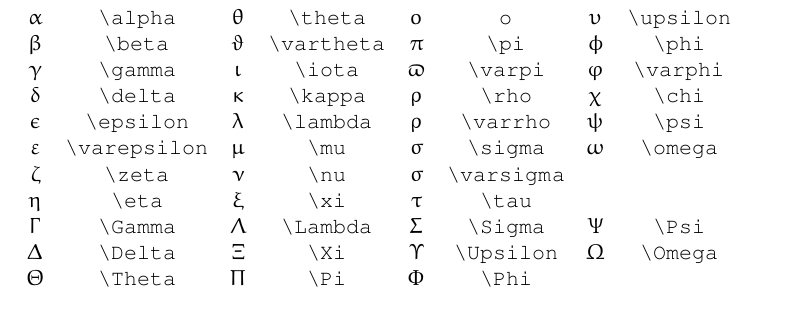
\includegraphics[width=30em]{../../algs/algs_999_zapp/letters.png}

\end{document}





